\chapter{Co-located Collaboration in Immersive Virtual Environment}
\label{chapter:colocated_colab}
\minitoc

\section{Introduction}


\section{Immersive Multi-user Display}
\subsection{Stereoscopy}
\subsection{Visual Distortion}
Immersive Projection Displays provide a natural place for teamwork \citep{Johanson2002IWP} as they are usually shared by a group of people rather than a single user. However, most projection-based displays can only support one fully tracked active user, other co-located users share the same point of view with distorted images and participate passively in the collaborative task \citep{Bayon2006Multiple}. This visual distortion impedes users' collaborative spatial judgments by impacting the perception of depth and direction in the virtual world \citep{Pollock2012Right}.

\subsection{Image Seperation Techniques}
To avoid visual distortion, different approaches have been explored to provide individual stereoscopic views for multiple co-located users with projection-based display. For example, Simon proposed a multi-viewpoint images technique \citep{Simon2007MVI} which projects different images from multiple viewpoints corresponding to the viewing positions of multiple users, and combines them to a single image on the screen. Users can only get a correct stereoscopic view from predefined position without head tracking, so with static images the interactions that they can have are limited. 

In order to have relatively large separate adaptive stereoscopic images for multiple users, time-multiplexing techniques become a working solution. Efforts have been made since 1997, for example, \citet{Agrawala1997TRW} designed a prototype of a responsive workbench to provide two tracked users with independent stereoscopic views without distortion. Later on, \citet{Kunz2002TSC} used a pair of shuttered LCD projectors to generate an active stereo display and then \citet{Frohlich2005MultiViewer} extended this shuttered display to support two to four users with better performance in terms of perceived flicker, brightness of each view and crosstalk. This technique makes it possible for a single screen to support more than one stereoscopic view. Images for different users are separated by active shutter glasses while the separation of the images for the left and right eye is ensured by passive polarized filters. In 2011, \citet{Kulik2011CSS} even developed a projection-based stereoscopic display for six users by using six customized DLP projectors. With each user having an independent stereoscopic view combined with real-time head tracking, more complex collaboration scenarios can be implemented for a group of co-located users.

Besides the development of display technology, various interaction techniques have also been proposed to make co-located collaboration in multi-user projection-based systems easier and more efficient, such as the see-through techniques \citep{Argelaguet2010STT}. However, these interaction techniques focus solely on situations where users are side-by-side. Direct face-to-face collaboration in projection-based display system is supposed to be impossible \citep{Salzmann2009CIC}. Therefore here we tried to study the possibility of having co-located face-to-face collaboration by investigating users' reaction to the perceptual conflicts raised with the dual-presence of the avatar and the real person.

\subsection{Summary}

\section{Co-located Collaboration}
\subsection{Reference Frame System}
Large projection-based displays can be an effective solution to support co-located collaboration in immersive CVEs. Especially, with the multi-stereoscopic projection-based setup as used by \citet{Salzmann2009VRPointing}, multiple users can collaborate side-by-side and interact with a virtual object in front of them with individual stereoscopic views of the virtual scene. However, as indicated by \citet{Salzmann2009CIC}, certain tasks that require face-to-face interaction between users cannot be applied directly within projection-based displays due to occlusions if an object is located in the middle of the users. In this case, if we want to benefit from the advantages of co-located collaboration in projection-based multi-stereoscopic systems for face-to-face tasks as in the side-by-side situations, we should prevent the users from working directly with each other.

Thus a possible solution is to introduce an avatar animated by real-time body motion capture for each user, and let each user work with the other users' avatars instead of the real person. In this case users' spatial relationship (relative position and orientation) in the virtual world is no longer constrained by the one in the physical workspace, they can be facing each other in the virtual world while physically side-by-side. This avatar-based approach enables complicated tasks that require both face-to-face and side-by-side interactions in projection-based multi-user system. For example, a car assembly task may contain two phases: during the first phase, users are on the same side of the model. They discuss and work together to repair a specific part of the car. Then in the second phase, they need to be at opposite sides of the car, and consequently have different viewpoints in the virtual world. Within this scenario one user can guide the other to properly fix a seat within the car cockpit. So with our avatar-based approach, they can switch between different spatial configurations without interrupting the ongoing task by using virtual navigation techniques.

However, with the solution proposed above, sometimes users may still enter each other's field of view when they work with the avatars. What is more, during a collaborative task, the communications between collaborators are usually conducted in a multimodal way \citep{Paggio2005Multimodal, Ennis2010Seeing} including verbal and non-verbal modalities \citep{Bailenson2002Gaze, Dodds2011Talk}, especially deictic gestures to refer to objects or places. So during a two-user co-located collaboration scenario, with the dual-presence of virtual and real information, users having multimodal interactions may encounter different perceptual conflicts both in the visual and audio modalities. For example (see Figure~\ref{fig:2_inconsistency}(a)), if user B points to an object for user A (from user B's viewpoint, he/she is pointing at a cube), user A may be confused by seeing both user B and his/her avatar doing the pointing gesture, and it may be problematic when there is another virtual object in the pointing direction of user B. Furthermore, normally the verbal communication between co-located users is conveyed by direct conversation without using headphones. As shown in Figure~\ref{fig:2_inconsistency}(b), user A is interacting with user B's avatar, but the vocal information comes from the real user B in a different direction. This kind of visual-audio inconsistency \citep{Di2009Recalibration, Spence2013Just} may be disturbing for users to concentrate on their collaboration.

\begin{figure}[tb]
  \centering
  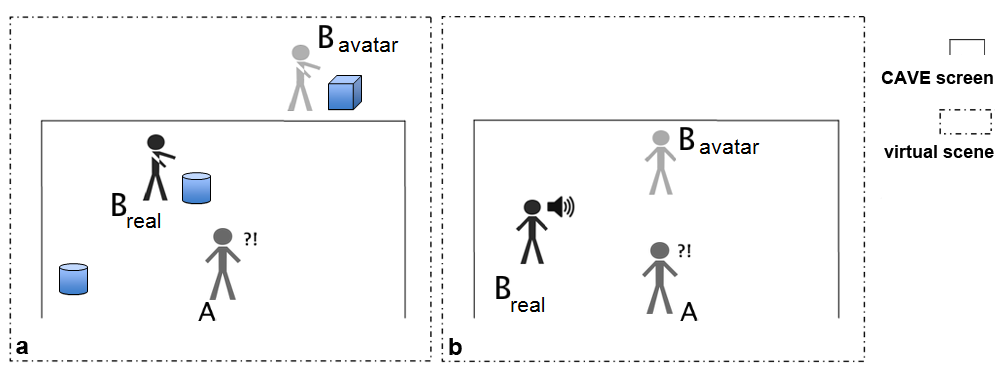
\includegraphics[width=\textwidth]{figures/ch2/inconsistency}
  \caption{\label{fig:2_inconsistency}Illustration of perceptual conflicts with a two-user scenario; user A interacts with avatar of user B: (a) Visual conflict occurs when user A simultaneously perceives the real user B and B's avatar pointing to different virtual objects. (b) Visual-audio conflict occurs when user B and the avatar are not at the same position.}
\end{figure}


\subsection{Spatial Collocation}
With multi-stereoscopy technology, novel projection-based immersive systems now can support multiple users by providing each one with an independent stereoscopic view of the virtual scene. When users work face-to-face, they may have an incorrect view if objects are located between them. In this case, avatars can be introduced to enable face-to-face interaction in the virtual world whereas they are side-by-side in the real device. As a consequence, such multi-user systems provide the users with a new kind of perceptual immersion and related cognitive experiences, because users must handle both information from the real world (i.e., other users' bodies) and those from the virtual scene (i.e., other users' avatars) at the same time.

Avatars have been used as media for multi-user communication in both remote and co-located use of immersive CVE, but the dual-presence of users and their avatars in the same immersive device for face-to-face interaction has not yet been addressed. We do not intend to create such dual-presence to test user's preference between real person and the avatar, but to observe users' reaction to different perceptual conflicts and to study if our avatar-based approach is sufficient to support face-to-face co-located collaboration in a multi-stereoscopic immersive display system.

Besides the development of display technology, various interaction techniques have also been proposed to make co-located collaboration in multi-user projection-based systems easier and more efficient, such as the bent pick ray \citep{Riege2006Bent} and the see-through techniques \citep{Argelaguet2010STT}. However, these interaction techniques focus solely on situations where users are side-by-side. Direct face-to-face collaboration in projection-based display system is supposed to be impossible \citep{Salzmann2009CIC}. Therefore here we tried to study the possibility of having co-located face-to-face collaboration by investigating users' reaction to the perceptual conflicts raised with the dual-presence of the avatar and the real person.


\section{Addressed Issues}
\subsection{Perceptual Conflicts}


\subsection{Navigation in Limited Workspace}
A lot of navigation techniques of different nature exist to allow users to travel through large virtual space, while physically stay within a limited workspace. These navigation techniques can be classified according to the control law - how a given input from the user can be mapped to a position or velocity change in the virtual world. Typical control laws include position and rate control, and can be implemented by both hardware and software solutions.

The most studied position control is natural walking, which is considered to be the most intuitive way to explore the virtual environment \citep{Ruddle2009BW}. To enable infinite walking in restricted real workspace, one can use both physical locomotion devices like treadmills \citep{Iwata1999Treadmill} and software solutions (e.g. redirection \citep{Peck2008RED}, resetting \citep{Williams2007ELV} and scaling techniques \cite{Interrante2007SLB}). Besides natural walking, walk-in-place \citep{Razzaque2002RWP} and WIM (World-In-Miniature) \citep{Stoakley1995VRW} are also interesting alternatives. Moreover, \citet{Fleury2010Generic} proposed a general model to integrate physical workspace into the virtual world and make the user aware of the physical environment in different ways. \citet{Cirio2012Cube} also summarized several metaphors for safe navigation in a restricted cubic workspace.

Conversely to previous techniques, rate control techniques are based on a virtual vehicle model which enables navigation in large virtual scenes. Users control directly the vehicle's velocity instead of position in the virtual world and can have the sensation of moving (self-motion illusion or vection \citep{Riecke2012Vection}). Actually the virtual vehicle can be controlled by information coming from different sources, for example, various input devices like joystick, haptic arm \citep{Martin2012Forklift} or even specific locomotion devices \citep{Marchal2011JOYMAN}. With video cameras or optical tracking systems, users can specify the velocity of the vehicle by motion tracking data of the hand (camera-in-hand \citep{Ware1990EVC}) or head movements \citep{Bourdot2002HCNav}. Gestures \citep{Konrad2003Gesture} and postures \citep{Kapri2011Steering} can also be used to move the virtual vehicle. Bowman et al. named this kind of virtual navigation techniques steering metaphors \citep{Bowman2004UIT} which are often relatively easy to implement and can provide efficient and flexible control of virtual navigation.

Some navigation metaphors such as the bubble technique \citep{Dominjon2005Bubble} and the magic barrier tape \citep{Cirio2009MBT} combine both position and rate control in order to enable infinite navigation within restricted real workspace. Position control is used within the physical workspace and then rate control is applied to the virtual vehicle to move further in the virtual world.


It is essential to keep user's safety when immersed in the virtual world. The navigation technique should prevent users from reaching the limits of the physical workspace. Some navigation metaphors such as the bubble technique \citep{Dominjon2005Bubble} and the magic barrier tape \citep{Cirio2009MBT} combine both walking and vehicle-based control in order to enable infinite navigation within restricted real workspace. \citet{Cirio2012Cube} summarized several metaphors for safe navigation in a restricted cubic workspace. Moreover, \citet{Fleury2010Generic} proposed a general model to integrate physical workspace into the virtual world and make the user aware of the physical environment in different ways.

\subsection{User Cohabitation}
Immersive virtual environment has the power to bring users to an artificial world by blocking the perception of the real world. In such situation users often forget boundaries of the physical workspace due to visual immersion, which could endanger both the user and the device. For some devices with non-closed display such as large image wall or a 3-wall CAVE, immersion is limited to the display area.

The human joystick metaphor does not necessarily prevent users from running into physical obstacles or keep user's field of view within projected areas. Moreover, if multiple users share the same immersive device for co-located collaboration with each one using a human joystick metaphor, they may have user cohabitation problems: users may run into collision when they move around without paying attention to other users (Figure~\ref{fig:2_illustration} left); one can also disrupt the visual perception of the virtual world of another if the former appears to be in the field of view of that user due to body occlusion (Figure~\ref{fig:2_illustration} right).

\begin{figure*}[tb]
  \centering
  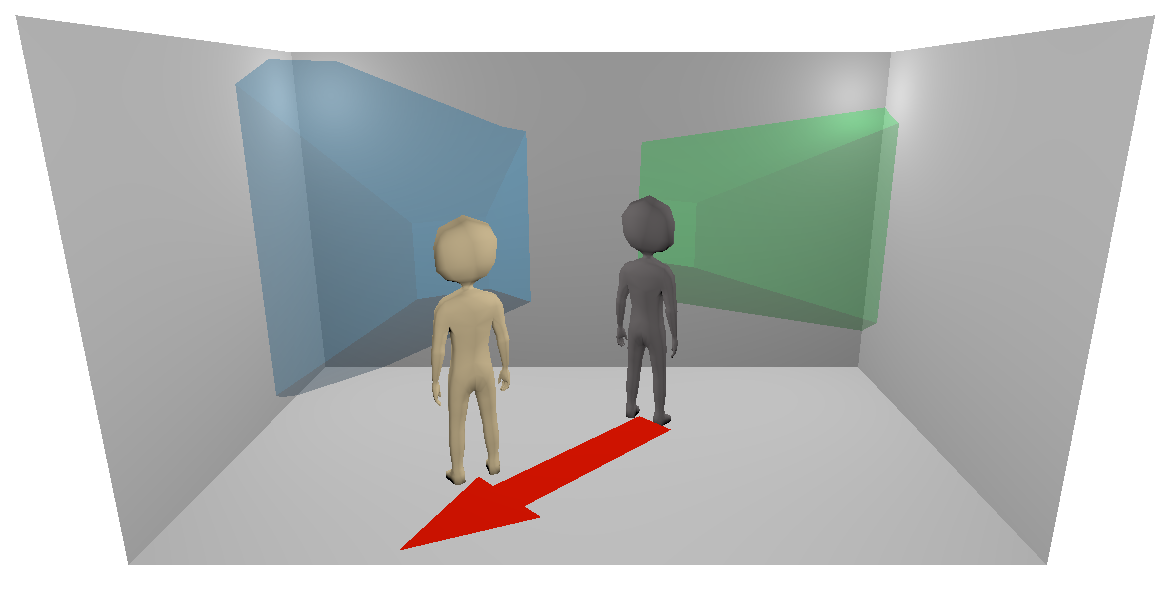
\includegraphics[width=0.49\textwidth]{figures/ch2/illu_col}
  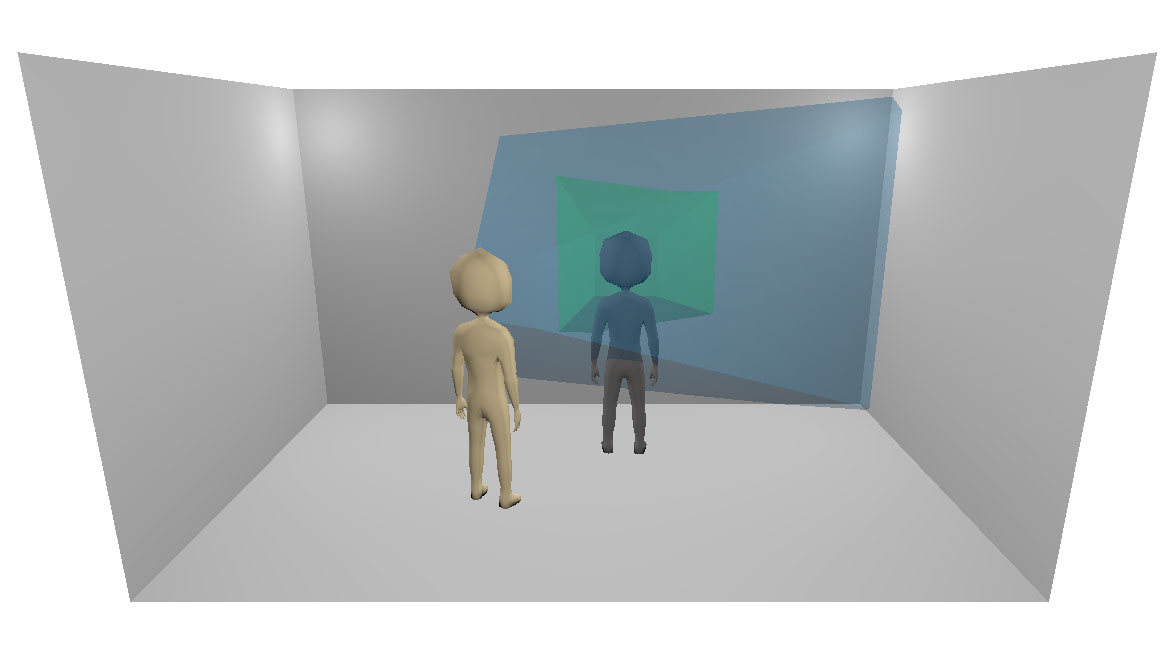
\includegraphics[width=0.49\textwidth]{figures/ch2/illu_occ}
  \caption{\label{fig:2_illustration}Illustration of collision (left) and occlusion (right) between co-located users in a multi-stereoscopic 3-wall plus floor CAVE.}
\end{figure*}

So to support safe and functional free navigation in an immersive context, the original human joystick metaphor should be adapted according to the number of co-located users and the configuration of the immersive system (size and shape of the screen walls, effective tracking space, etc.).

Two aspects of the problem should be solved: how to manage the spatial relationship between active users and the immersive display boundaries, i.e. how to prevent users from touching the wall screens and from seeing non projected areas, and how to provide enough workspace for each co-located user and thus avoid collision and occlusion between them.

When it comes to managing multiple users in the same immersive virtual environment for co-located collaboration, most works focused only on closely coupled collaboration (e.g. co-manipulation). In this case, virtual navigation is either disabled or controlled by a leader and shared by other users \citep{Beck2013IGG, Kulik2011CSS}. To enable more complex collaborative scenarios including loosely coupled tasks which require individual navigation for co-located users, we should propose novel navigation models that comply with user cohabitation constrains.

\subsection{Summary}

\section{Approach - Altered Human Joystick}

\subsection{Basic Model}
The basic navigation method we use is a reduced version (from 6DoF to 3DoF) of a head-controlled navigation technique (Figure~\ref{fig:2_hcnav}) proposed by \citet{Bourdot2002HCNav}. It is actually a human joystick metaphor \citep{McMahan2012EDF}, but with an additional degree of freedom for yaw rotation. User's head position and orientation are captured in real time with an optical tracker attached to the 3D glasses.

To navigate, user first needs to choose a neutral reference frame (composed of a position and an orientation ($P_{0}, \theta_{0}$)) during calibration. Then user can move in the real workspace relatively to this reference frame to control the linear and angular velocity of the vehicle ($\overrightarrow{v_{veh}}, \Omega_{veh}$), denoting $(P, \theta)$ the current configuration. The translation and rotation gain functions are configured respectively by coefficients $K_{T}$ and $K_{R}$.

\begin{equation}
\overrightarrow{v_{veh}}=K_{T}\cdot \overrightarrow{P_{0}P}
\end{equation}
\begin{equation}
\overrightarrow{\Omega_{veh}}=K_{R}\cdot \widehat{\theta_{0}\theta}
\end{equation}

\begin{figure}[tb]
  \centering
  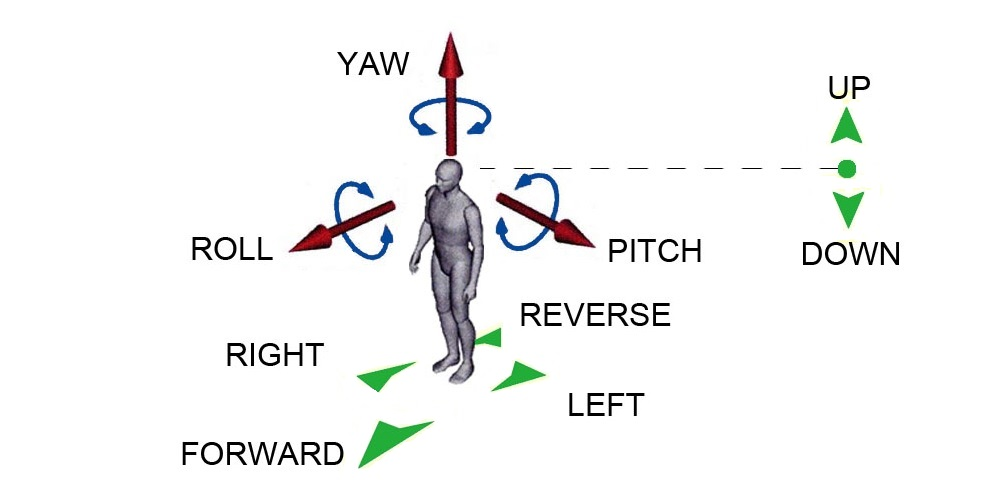
\includegraphics[width=0.8\textwidth]{figures/ch2/HCNav}
  \caption{\label{fig:2_hcnav}Head-controlled navigation paradigm.}
\end{figure}

\subsection{Alterations}

\subsubsection{Altered Gain Function}
 To restrain user's translational workspace, we can replace the linear gain function with a divergent one integrating the distance limitation into the navigation model.

\begin{equation}
\overrightarrow{v_{veh}}=K_{T}\cdot \left(\frac{\Delta x}{X_{m}-\Delta x},\:\frac{\Delta y}{X_{m}-\Delta y}\right)
\end{equation}

where $X_{m}$ is the minimum distance from the neutral position $P_{0}$ to the border of the physical system (Figure~\ref{fig:2_workspace_border}a). This divergent gain function allows user to apply an infinite vehicle velocity when reaching $X_{m}$. So the workspace of a user is defined by the physical space that user is free to move inside before reaching any borders.

\begin{figure}[tb]
\begin{center}
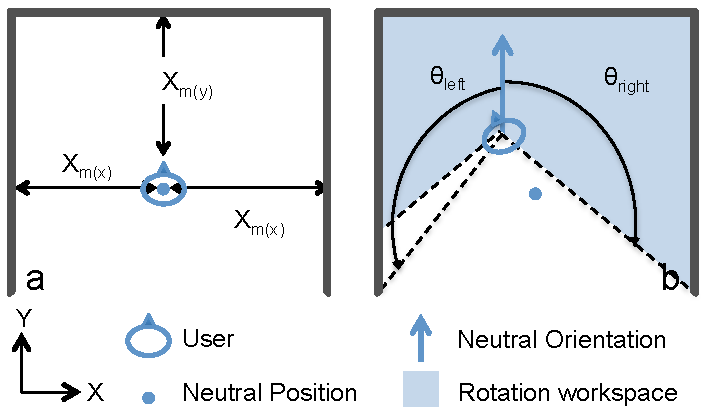
\includegraphics[width=0.6\textwidth]{figures/ch2/workspace_border}
\par\end{center}
\caption{\label{fig:2_workspace_border}(a) The maximum available workspace $X_{m}$ can have different values on x and y axis. (b) User's rotational workspace is defined by $\theta_{max}$ on both sides of the neutral orientation.}
\end{figure}

To avoid collision between users, we can consider each user as a moving border which restricts directly the workspace of other users. However, this method makes the velocity control too unstable when all users move the same time. A possible compromised solution is to assign each user a safe zone for proper use, and an overlapped zone to share with others. We adjust the ``virtual border" of one user's workspace depending on the penetration of other users in the shared area. This way a user's velocity will only be influenced by others when he/she is inside the shared zone, one can make use of the entire shared zone as if he/she was alone in the system until the other user also needs to use it. Figure~\ref{fig:2_adaptive_trans_border} shows an example of two users inside a 3-wall CAVE system. Usually CAVE-like systems are in a rectangular form, so the border formed by a user is chosen to be a vertical plane.

\begin{figure}[tb]
\begin{center}
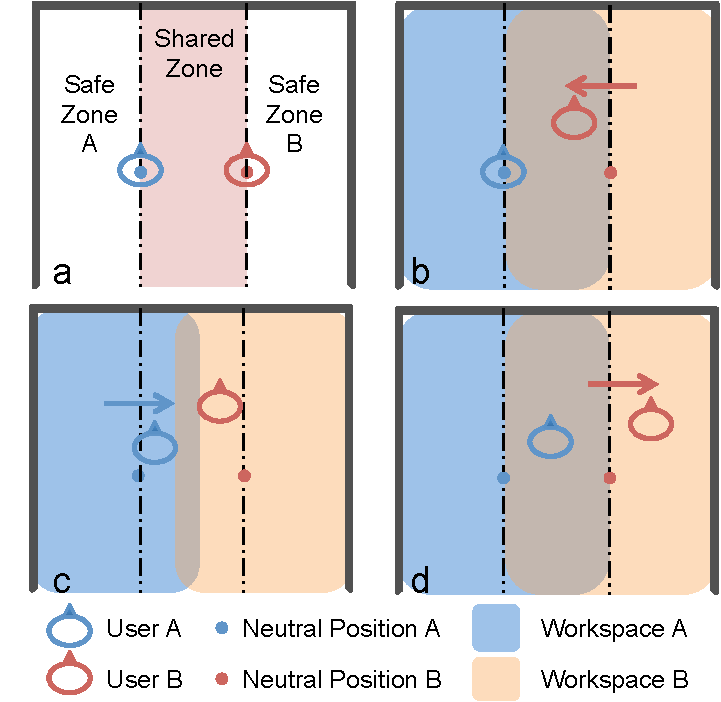
\includegraphics[width=0.6\textwidth]{figures/ch2/adaptive_trans_border}
\end{center}
\caption{\label{fig:2_adaptive_trans_border}Adaptive border of user's workspace for translation in a two-user case : a) Initial state. b) User B moves into the shared zone while user A is still in the safe zone, both users' workspaces are not influenced and user B can use the entire shared zone. c) User A also moves into the shared zone and pushes the border of user B's workspace to the right. d) User B moves back to the safe zone, the entire shared zone can now be used by user A.}
\end{figure}

Considering rotations, physical constrains could also be integrated into the gain function similarly as for translation. For example, in a 3-wall CAVE it is preferable to avoid user occlusions and prevent users from seeing the empty screen behind them. However, due to the different nature between translation and rotation movements, we chose to use a saturated quadratic gain function rather than a divergent form as follows:

\begin{equation}
\Omega_{veh}=
  \begin{cases}
    \frac{\Omega_{max}}{(\theta_{max})^{2}}\cdot(|\Delta\theta|)^{2} & \text{if } |\Delta\theta|<\theta_{max} \\
    \Omega_{max} & \text{if } |\Delta\theta| \geq \theta_{max}
  \end{cases}
\end{equation}

where $\theta_{max}$ represents the maximum available rotational workspace (with which the user reaches the maximum rotation speed $\Omega_{max}=\pi\, rad.s^{-1}$) computed as the minimum of $\theta_{left}$, $\theta_{right}$ and $\theta_{user}$ to provide a symmetric vehicle control around the neutral orientation $\theta_{0}$ (Figure~\ref{fig:2_workspace_border}b).  


\subsubsection{Adaptive Neutral Reference Frame}

The original human joystick metaphor has a fixed neutral reference frame (a neutral position and orientation) defined during calibration. This reference frame should give user the maximum workspace that the physical working environment can offer, for example, the center of a CAVE is often a good choice. However, when we have mobile obstacles in the physical working environment, e.g. multiple co-located users, it may be inappropriate to have a fixed reference frame. With the above methods of computing user's available workspace, a fixed neutral reference frame distribution will often lead to non-symmetric use of the total available workspace both for translation and rotation.

To optimize workspace usage, we can reconfigure each user's neutral reference frame as the center of his/her available workspace (Figure~\ref{fig:2_neutral_ref}). In this way, each user's workspace is balanced between constrains introduced by the display system and by other users, and is always symmetric on the left and right with respect to the neutral reference frame.

Although this method could make better use of the total workspace, it also potentially increases the mutual influence between users, which may be disturbing for the navigation control. When users have relatively small workspace, the variation of neutral reference frame may remain imperceptible during navigation, which is to be tested.   

\begin{figure}[tb]
  \centering
  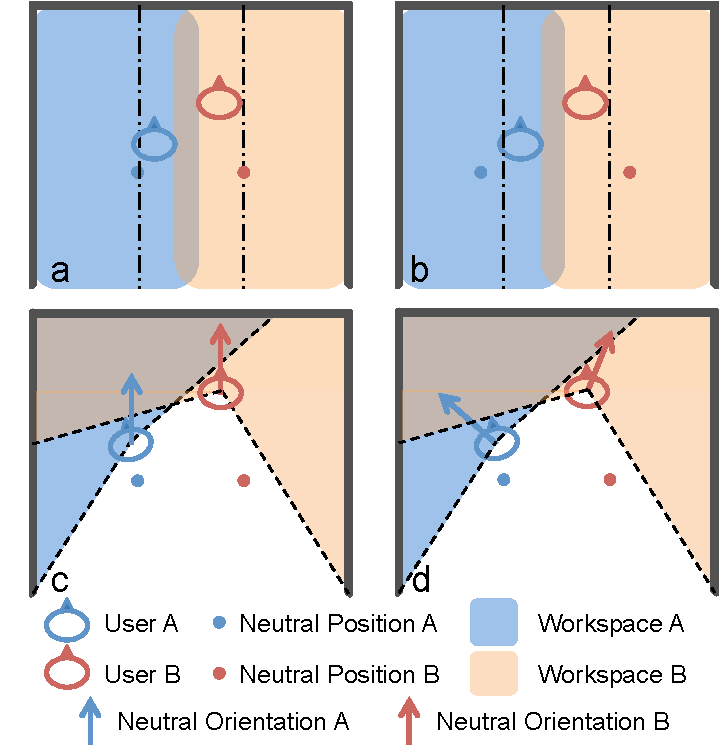
\includegraphics[width=0.6\textwidth]{figures/ch2/neutral_ref}
  \caption{\label{fig:2_neutral_ref}(a, c) Users' neutral reference frames are fixed to the initial distribution. (b, d) Users' neutral reference frames are computed dynamically according to both users' positions.}
\end{figure}



\section{Chapter Summary}



